\section{内核功能实现}\label{sec:KernelFunctionalityImplementation}

内核是操作系统的核心组件,负责管理内存和设备,同时为软件应用程序提供使用这些资源的接口。根据复杂性和目标的不同,内核的开发可以遵循不同的模型。主要有两种模型:微内核\footnote{微内核是一种操作系统内核设计,其核心理念是将内核功能最小化,只保留最基本的操作系统服务,如最低级的内存管理、进程调度和通信机制。其他更复杂的服务,如文件系统、网络协议、设备驱动等,则运行在用户空间。}和宏内核\footnote{宏内核则是传统的内核设计方式,将大部分的系统服务和管理功能,如设备驱动、文件系统管理、网络服务等,都直接在内核空间内实现。}。微内核的目标是将大多数服务运行在用户空间,从而提高安全性和模块化。

MinmusOS 采用的是宏内核模式,因此其所有服务和设备驱动程序都在单一地址空间内运行,并处于特权模式下。这种模式提高了效率并减少了代码复杂性,但缺点是其中任何一个组件的错误都可能导致整个系统崩溃。

在本节(\cref{sec:KernelFunctionalityImplementation})中,笔者将详细探讨 MinmusOS 内核各项功能的实现,包括中断管理、驱动程序、多任务处理、系统调用、命令行解释器、内存管理以及文件系统。

\subsection{中断(Interrupts)}

中断是操作系统中关键的概念之一,主要用于处理外部设备的信号或内部事件。中断机制使得CPU可以响应并处理紧急事件,同时保持对其他任务的执行。中断主要分为三种类型:

\begin{enumerate}
    \item \textbf{异常(Exceptions)}:同步中断,由CPU执行指令过程中的事件或错误引发,例如除以零错误、执行非法指令或访问无效内存地址。异常通常分为两类:可屏蔽异常和不可屏蔽异常。可屏蔽异常允许操作系统根据当前的需求和优先级来决定是否立即处理。
    \item \textbf{硬件中断(Hardware Interrupts)}:异步中断,由外部硬件设备产生,例如键盘输入、鼠标移动或网络数据包到达。硬件中断使得设备可以通知CPU它们需要立即处理的事件,这对于实时数据处理非常重要。
    \item \textbf{软件中断(Software Interrupts)}:由执行特定的CPU指令集(如INT指令)显式触发,常用于操作系统的系统调用,比如文件访问、网络通信或其他服务请求。软件中断还可以用来执行BIOS(基本输入输出系统)例程,或者其他低级操作。
\end{enumerate}

当中断发生时,CPU会采取以下步骤来处理:

\begin{enumerate}
    \item \textbf{保存当前状态}:CPU首先保存当前正在执行的任务的状态,以便中断处理完成后可以恢复。
    \item \textbf{识别中断类型}:CPU通过查询中断向量表(一个存储了所有中断处理程序入口地址的表格)来识别中断的具体类型和来源。
    \item \textbf{执行中断服务例程(ISR,Interrupt Service Routine)}:每种中断类型都有对应的服务程序。CPU执行这些程序来处理中断。
    \item \textbf{恢复状态}:中断服务完成后,CPU恢复之前中断的任务状态,继续之前的操作。
\end{enumerate}

中断处理机制的设计对于操作系统的效率和响应时间至关重要。优秀的中断处理策略可以显著提高系统的整体性能和用户体验。

\subsubsection{中断描述符表(Interrupt Descriptor Table)}

中断描述符表(IDT)是x86架构中特有的一个关键数据结构,用于管理中断的处理。它的主要目的是提供一个中断服务例程(ISR)的地址映射,当中断发生时,CPU能够知道跳转到哪个位置执行相应的中断处理程序。

IdtEntry 是中断描述符表(IDT)中的基本单元,它定义了每个中断处理函数的具体属性和位置。IdtEntry 结构体的定义如\cref{lst:IdtEntryDataStructure}所示。\texttt{\#[derive(Copy, Clone, Debug)]} 使用 derive 宏为结构体自动实现 Copy、Clone 和 Debug 这三个 trait,\texttt{\#[repr(C, packed)]} 用于指定结构体使用 C 语言风格的内存布局并取消字段对齐,以确保字段在内存中紧凑排列。

\begin{listing}[htbp]
    \begin{minted}{rust}
#[derive(Copy, Clone, Debug)]
#[repr(C, packed)]
pub struct IdtEntry {
    offset_low: u16,       // 偏移地址的低 16 位
    segment_selector: u16, // 中断处理程序代码所在的段选择器
    reserved: u8,          // 保留字段,设置为 0
    flags: u8,             // 位标志
    offset_high: u16,      // 偏移地址的高 16 位
}
    \end{minted}
    \caption{\texttt{IdtEntry}数据结构}\label{lst:IdtEntryDataStructure}
\end{listing}

位标志,包含门类型(Gate Type)、DPL(Descriptor Privilege Level)和 P(Presence):

\begin{enumerate}
    \item \textbf{门类型(Gate Type)}:决定IDT条目是中断门还是陷阱门。例如,0xE(1110b)代表32位中断门。
    \item \textbf{DPL(Descriptor Privilege Level)}:指定可以调用中断的最低特权级(CPL),通常为0,表示只有内核模式可以使用。
    \item \textbf{P(Presence)}:此位必须设置为1,表示此中断向量是有效的。
\end{enumerate}

IdtEntry 结构体提供了 set 方法(\cref{lst:IdtEntrySetMethod})用于设置中断处理程序的地址,这个方法接受一个32位的整数 offset,代表中断处理程序的地址。然后将这个地址分解为两个16位的部分,分别存储到 offset\_low 和 offset\_high。

\begin{listing}[htbp]
    \begin{minted}{rust}
pub fn set(&mut self, offset: u32) {
    self.offset_low = ((offset << 16) >> 16) as u16;
    self.offset_high = (offset >> 16) as u16;
}
    \end{minted}
    \caption{\texttt{IdtEntry}的set方法}\label{lst:IdtEntrySetMethod}
\end{listing}

IdtDescriptor 结构体(\cref{lst:IdtDescriptorDataStructure})定义了一个用于加载中断描述符表(IDT)的描述符。它用于指定 IDT 的大小和内存中的位置,从而允许处理器正确地找到并使用 IDT。size 表示 IDT 的大小,但实际上是 IDT 中最后一个有效条目的偏移量加一。因为中断向量表的条目索引从 0 开始,所以 size 字段的值等于 IDT 的字节长度减一。offset 是一个指向 InterruptDescriptorTable 的指针,表示 IDT 的起始物理地址。这个指针告诉处理器从哪里开始读取中断向量表的数据。

\begin{listing}[htbp]
    \begin{minted}{rust}
#[repr(C, packed)]
pub struct IdtDescriptor {
    size: u16,
    offset: *const InterruptDescriptorTable,
}
    \end{minted}
    \caption{\texttt{IdtDescriptor}数据结构}\label{lst:IdtDescriptorDataStructure}
\end{listing}

InterruptDescriptorTable 结构体(\cref{lst:InterruptDescriptorTableDataStructure})实现了一个关键的系统级数据结构,即中断描述符表(IDT)。这个表是操作系统中管理中断向量的核心结构,用于定义每个中断或异常的处理程序地址。

\begin{listing}[htbp]
    \begin{minted}{rust}
#[repr(C, packed)]
pub struct InterruptDescriptorTable {
    entries: [IdtEntry; IDT_ENTRIES],
}

impl InterruptDescriptorTable {
    pub fn init(&mut self) {
        for i in 0..IDT_ENTRIES {
            self.add(i, exceptions::generic_handler as u32);
        }
    }

    pub fn add(&mut self, int: usize, handler: u32) {
        self.entries[int].set(handler);
    }

    pub fn load(&self) {
        let descriptor = IdtDescriptor {
            size: (IDT_ENTRIES * size_of::<IdtEntry>() - 1) as u16,
            offset: self,
        };
        unsafe {
            asm!("lidt [{0:e}]", in(reg) &descriptor);
        }
    }

    pub fn add_exceptions(&mut self) {
        self.add(0x00, exceptions::division_error as u32);
        ...
        self.add(0x15, exceptions::control_protection_exception as u32);
    }
}
    \end{minted}
    \caption{\texttt{InterruptDescriptorTable}数据结构}\label{lst:InterruptDescriptorTableDataStructure}
\end{listing}

中断描述符表(IDT)的结构体定义与方法实现:

\begin{enumerate}
    \item \textbf{结构体定义}:entries 包含了 IDT\_ENTRIES(256)数量的 IdtEntry 结构体实例。每个 IdtEntry 对应一个中断向量,存储中断处理程序的具体位置和相关属性。
    \item \textbf{init方法}:初始化 IDT 的每个条目,将所有中断向量的处理程序设置为一个通用的处理函数 \texttt{exceptions::generic\_handler}。
    \item \textbf{add方法}:设置特定中断向量的处理程序。它接受中断向量的索引和处理程序的地址(函数指针),然后调用 IdtEntry 的 set 方法来更新相应的条目。
    \item \textbf{load方法}:将 IDT 加载到 CPU 的 IDT 寄存器。它创建一个 IdtDescriptor 结构体,该结构体包含了 IDT 的大小和地址,然后使用 lidt 汇编指令加载这个描述符。
    \item \textbf{add\_exceptions方法}:为常见的 CPU 异常配置特定的处理程序,如除零错误、无效操作码、双重故障、通用保护和页面错误等,中断向量表见\cref{tab:InterruptVectorTable}。
\end{enumerate}

IDT\_ENTRY 是 IdtEntry 类型的静态变量,\cref{lst:IdtEntryTemplate}定义了一个默认的 IDT 条目模板。这个模板被用来初始化 IDT 数组中的每个条目。

\begin{listing}[htbp]
    \begin{minted}{rust}
pub static IDT_ENTRY: IdtEntry = {
    // 段选择器,确定中断处理程序的代码段
    let segment_selector: u16 = {
        let rpl = 0b00 << 0;       // 请求特权级(Ring Privilege Level),0 表示最高权限级别
        let ti = 0b0 << 2;         // 表指示符(Table Indicator),0 表示使用全局描述符表(GDT)
        let index = 0b1 << 3;      // GDT 中的索引,这里是 0x8
        rpl | ti | index           // 组合成完整的段选择器
    };

    // 保留字段,必须设为 0
    let reserved: u8 = 0;

    // 标志位字段,定义了 IDT 条目的属性
    let flags: u8 = {
        let gate_type = 0xe << 0;  // 门类型,0xE 表示 32 位中断门,0xF 表示 32 位陷阱门
        let zero = 0 << 3;         // 保留位,必须为 0
        let dpl = 0 << 5;          // 描述符特权级,0 表示只有内核模式可以使用此中断
        let p = 1 << 7;            // 存在位(Presence bit),1 表示此中断有效
        gate_type | zero | dpl | p // 组合成完整的标志位
    };

    // 构造 IdtEntry 结构体实例
    IdtEntry {
        offset_low: 0,             // 中断处理程序的低 16 位地址,初始化设置为 0,后续指定具体值
        segment_selector,          // 上面定义的段选择器
        reserved,                  // 保留位,始终为 0
        flags,                     // 标志位,定义了 IDT 条目的特性
        offset_high: 0,            // 中断处理程序的高 16 位地址,初始化设置为 0,后续指定具体值
    }
};
    \end{minted}
    \caption{IDT 条目模板}\label{lst:IdtEntryTemplate}
\end{listing}

IDT 是 InterruptDescriptorTable 类型的静态变量,它实际上是一个包含 256 个 IdtEntry 条目的数组。这个数组构成了整个中断描述符表,用于响应各种中断请求。\cref{lst:IDT}使用 IDT\_ENTRY 来初始化每个元素,这意味着每个条目初始时都复制了 IDT\_ENTRY 的设置。特定的中断向量将通过调用 InterruptDescriptorTable 的 add 方法来设置特定的处理函数。

\begin{listing}[htbp]
    \begin{minted}{rust}
pub static mut IDT: InterruptDescriptorTable = InterruptDescriptorTable {
    entries: [IDT_ENTRY; IDT_ENTRIES]
};
    \end{minted}
    \caption{中断描述符表}\label{lst:IDT}
\end{listing}

IDT 定义了操作系统如何响应硬件和软件生成的中断。每个条目对应一个中断向量,系统在收到中断时会查询 IDT 以确定如何处理该中断。通过提供一个统一的方式来处理所有类型的中断,操作系统能够更加有效地管理资源和响应外部事件,从而增强系统的稳定性和响应性。

\subsubsection{中断服务例程(Interrupt Service Routines)}

中断服务例程(ISR)是一种特定的程序,用于处理来自硬件或软件的中断信号。当系统发生中断时,CPU 会自动查找中断描述符表(IDT)中相应的服务例程,并跳转到该例程执行相关操作。与普通的 C 函数不同,ISR 由 CPU 直接调用,并使用特定的 iret 指令返回,这种指令用于恢复中断前的状态,确保系统能安全地继续执行其他任务。

在编写 ISR 时,需要特别注意 CPU 在调用中断服务例程之前会自动将一些寄存器的值压栈,这些寄存器包括 EFLAGS、EIP 和 CS。EFLAGS 寄存器包含了系统的状态标志,EIP 是程序计数器,指示下一条执行指令的地址,CS 是代码段寄存器,指示当前执行代码的段基址。

大部分操作系统使用专门的汇编语言函数来实现中断处理程序,以确保处理过程的高效和准确。MinmusOS 采用 Rust 的内联汇编技术来实现 ISR。这种方法允许在中断服务例程中直接调用其他 Rust 函数,然后通过 iret 指令安全返回,这种技术的使用使得中断处理程序既可以保持高效,也能利用 Rust 语言的安全特性。

\begin{listing}[htbp]
    \begin{minted}{rust}
#[naked]
pub extern "C" fn generic_handler() {
    unsafe {
        asm!(
        "push 0xFF",              // 向堆栈推送一个错误代码
        "call exception_handler", // 调用 exception_handler 函数,用于显示错误信息并处理中断
        "add esp, 4",             // 调整堆栈指针,以清除之前压入的错误代码
        "iretd",                  // 使用中断返回指令,恢复之前由 CPU 自动保存的状态
        options(noreturn),        // 表明汇编代码块执行后不会返回到原始的 Rust 函数中
        );
    }
}
    \end{minted}
    \caption{通用中断处理器}\label{lst:GenericHandler}
\end{listing}

\cref{lst:GenericHandler}定义了一个用于处理多种中断的通用中断服务例程(ISR)。使用 \texttt{\#[naked]} 属性表示这个函数没有由编译器生成的 prologue \footnote{函数的 prologue 是函数实际执行之前的准备阶段。在这个阶段,编译器或者程序会保存旧的基指针、设置新的基指针和为局部变量分配空间。}和 epilogue\footnote{函数的 epilogue 是函数执行完成后的清理阶段。在这个阶段,编译器或者程序会恢复堆栈指针、恢复基指针和返回到调用者。},使得函数可以完全控制所有的堆栈操作。这种处理方式对于中断处理程序来说是必要的,因为它们需要精确控制寄存器和堆栈的状态,但也增加了复杂性和出错的风险。

\begin{listing}[htbp]
    \begin{minted}{rust}
#[no_mangle]
pub extern "C" fn exception_handler(int: u32, eip: u32, cs: u32, eflags: u32) {
    unsafe {
        PRINTER.set_colors(COLOR_WHITE, COLOR_BLUE);
        PRINTER.clear();
    }
    lib::println!();
    lib::println!("  ========== MinmusOS v1.0 ==========                            By Jishen Lin");
    lib::println!();
    lib::println!("  SERIOUS KERNEL ERROR!");
    lib::println!();
    lib::println!("  MinmusOS has encountered a fatal error and the system has been halted.");
    lib::println!();
    lib::println!();
    lib::println!();
    lib::println!();
    lib::println!("  EXCEPTION DESCRIPTION:");
    lib::println!();
    match int {
        0x00 => {
            lib::println!("    DIVISION ERROR!");
        }
        ...
        _ => {
            lib::println!("    EXCEPTION!");
        }
    }
    lib::println!();
    lib::println!();
    lib::println!("  TECHNICAL INFORMATION:");
    lib::println!();
    lib::println!("    ERROR_CODE      : {}", int);
    lib::println!("    INSTRUCTION_PTR : 0x{:X}", eip);
    lib::println!("    CODE_SEGMENT    : 0x{:X}", cs);
    lib::println!("    EXTENDED_FLAGS  : 0b{:b}", eflags);
    lib::println!();
    lib::println!();
    lib::print!("  Please restart your computer. :)");
    loop {}
}
    \end{minted}
    \caption{异常处理器}\label{lst:ExceptionHandler}
\end{listing}

在调试过程中,在代码中通过内联汇编使用 int 命令可以手动触发中断。\cref{lst:ExceptionHandler}为 MinmusOS 提供了友好的用户交互(\cref{fig:ExceptionHandlerPresentation})。蓝屏界面采用了经典的蓝底白字风格,类似于传统的Windows蓝屏死机(BSOD),并显示了详细的错误信息,包括错误类型和技术信息(如错误代码、指令指针、代码段、扩展标志等),有助于开发人员定位问题,便于调试和修复。

\begin{figure}[htbp]
    \centering
    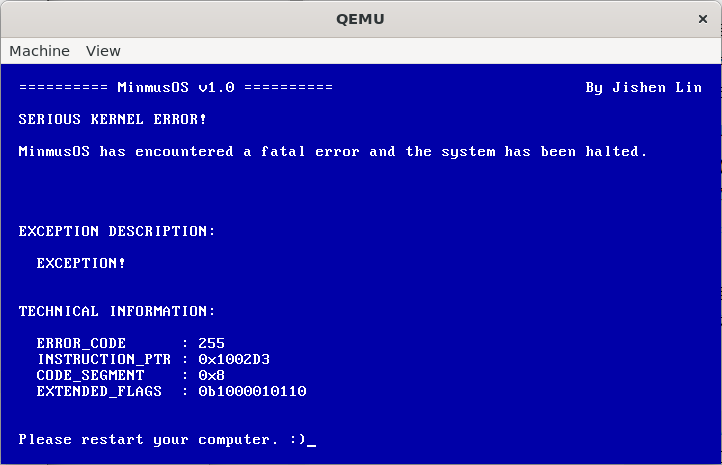
\includegraphics[width=0.8\textwidth]{figures/ExceptionHandlerPresentation.png}
    \caption{异常处理器演示}
    \label{fig:ExceptionHandlerPresentation}
\end{figure}

\subsubsection{CPU 异常(CPU Exceptions)}

异常是 CPU 在执行当前指令过程中遇到错误时自身触发的一种中断。在 x86 架构上,大约有 20 种不同的 CPU 异常类型,见\cref{tab:InterruptVectorTable}。\cref{tab:InterruptVectorTable} 参考自 Intel® 64 和 IA-32 架构软件开发者手册。

\begin{longtable}[c]{@{}llllll@{}}
    \caption{中断向量表}
    \label{tab:InterruptVectorTable}                                                                                                                                                                                                                  \\
    \toprule
    \textbf{向量} & \textbf{助记符} & \textbf{描述}                                                                                                                                            & \textbf{类型} & \textbf{错误代码} & \textbf{来源}                   \\ \midrule
    \endfirsthead
    \multicolumn{6}{r}{\textbf{续表~\thetable}}                                                                                                                                                                                                         \\
    \toprule
    \textbf{向量} & \textbf{助记符} & \textbf{描述}                                                                                                                                            & \textbf{类型} & \textbf{错误代码} & \textbf{来源}                   \\ \midrule
    \endhead
    \hline
    \multicolumn{6}{r}{续下页}
    \endfoot
    \endlastfoot
    0           & \#DE         & 除零错误                                                                                                                                                   & 故障          & 否             & DIV 和 IDIV 指令                 \\
    1           & \#DB         & 调试异常                                                                                                                                                   & 故障/陷阱       & 否             & 指令、数据和 I/O 断点;单步执行等           \\
    2           &              & NMI中断                                                                                                                                                  & 中断          & 否             & 不可屏蔽的外部中断                     \\
    3           & \#BP         & 断点                                                                                                                                                     & 陷阱          & 否             & INT3 指令                       \\
    4           & \#OF         & 溢出                                                                                                                                                     & 陷阱          & 否             & INTO 指令                       \\
    5           & \#BR         & BOUND 范围超出                                                                                                                                             & 故障          & 否             & BOUND 指令                      \\
    6           & \#UD         & 无效操作码(未定义操作码)                                                                                                                                          & 故障          & 否             & UD 指令或保留操作码                   \\
    7           & \#NM         & 设备不可用(无数学协处理器)                                                                                                                                         & 故障          & 否             & 浮点数或 WAIT/FWAIT 指令            \\
    8           & \#DF         & 双重故障                                                                                                                                                   & 中止          & 是(零)          & 任何能生成异常、NMI 或 INTR 的指令        \\
    9           &              & 协处理器段溢出(保留)                                                                                                                                            & 故障          & 否             & 浮点数指令                         \\
    10          & \#TS         & 无效的 TSS\footnote{TSS(Task State Segment)是Intel x86架构中用于任务切换和状态维护的数据结构。它存储了处理器在执行任务时需要的所有状态信息,使得操作系统能够管理多任务环境中的任务切换。TSS的使用主要体现在硬件级别的任务切换和保护模式下的任务状态管理。} & 故障          & 是             & 任务切换或 TSS 访问                  \\
    11          & \#NP         & 段不存在                                                                                                                                                   & 故障          & 是             & 加载段寄存器或访问系统段                  \\
    12          & \#SS         & 栈段故障                                                                                                                                                   & 故障          & 是             & 栈操作和 SS 寄存器加载                 \\
    13          & \#GP         & 通用保护                                                                                                                                                   & 故障          & 是             & 任何内存引用和其他保护检查                 \\
    14          & \#PF         & 页面错误                                                                                                                                                   & 故障          & 是             & 任何内存引用                        \\
    15          &              & (Intel 保留)                                                                                                                                             &             & 否             &                               \\
    16          & \#MF         & x87 FPU 浮点错误(数学故障)                                                                                                                                     & 故障          & 否             & x87 FPU 浮点或 WAIT/FWAIT 指令     \\
    17          & \#AC         & 对齐检查                                                                                                                                                   & 故障          & 是(零)          & 内存中的任何数据引用                    \\
    18          & \#MC         & 机器检查                                                                                                                                                   & 中止          & 否             & 错误代码(如果有)和来源取决于模型             \\
    19          & \#XM         & SIMD 浮点异常                                                                                                                                              & 故障          & 否             & SSE/SSE2/SSE3 浮点指令            \\
    20          & \#VE         & 虚拟化异常                                                                                                                                                  & 故障          & 否             & EPT 违规                        \\
    21          & \#CP         & 控制保护异常                                                                                                                                                 & 故障          & 是             & RET/IRET/RSTORSSP/SETSSBSY 指令 \\
    22-31       &              & (Intel 保留)                                                                                                                                             &             &               &                               \\
    32-255      &              & 用户定义(非保留)中断                                                                                                                                            & 中断          &               & 外部中断或 INT n 指令                \\ \bottomrule
\end{longtable}

\subsubsection{可编程中断控制器(Programmable Interrupt Controller)}

可编程中断控制器(Programmable Interrupt Controller,简称 PIC),尤指 8259 PIC,是早期计算机主板上用于管理硬件中断的一个小型芯片。在现代计算机中,这一芯片通常已被整合进 CPU 的设计中。PIC 的核心作用是接收来自硬件设备的中断信号,并在 CPU 准备接收时,将这些信号有效地分派给 CPU,从而响应外部设备的事件或请求。

PIC 有 28 个引脚,其中 8 个引脚是中断输入线,用于连接那些可以触发中断的硬件组件。这些中断线路将外部设备如键盘、鼠标或其他I/O设备的中断请求直接传输到 PIC。由于单个 PIC 只能处理有限的 8 个中断,现代计算机系统为了扩展中断处理能力,通常会使用两个 PIC 芯片,配置为一主一从模式。这种配置允许系统处理更多的中断线路,总共可达 15 个中断(一个用于连接主从 PIC)。虽然现代计算机系统普遍采用了更为先进的高级可编程中断控制器(APIC),以支持更大数量的中断线路和更复杂的中断管理功能,PIC 依旧因其向后兼容性而被支持在新的系统中,确保老旧硬件和软件的正常运行。

CPU 在设计时已经为处理器内部的异常(如除零错误、访问违规等)预留了前 32 个中断向量。因此,来自外部硬件的中断必须被映射到 32 号以上的中断向量,以避免与这些处理器异常冲突。

重新映射中断是通过向 PIC 的命令和数据端口发送特定的命令来完成的。对于主 PIC,其命令端口位于 0x20,数据端口位于 0x21;从 PIC 的命令端口位于 0xA0,数据端口位于 0xA1。初始化 PIC 时,会发送一个初始化命令,设定中断向量的偏移量,指定哪个是主 PIC,哪个是从 PIC,并设置运行模式。

可编程中断控制器(Programmable Interrupt Controller)驱动程序的实现见\cref{sec:ProgrammableInterruptControllerDriver}。

\subsection{驱动程序(Drivers)}

设备驱动程序是一种软件组件,其目的是使特定的硬件设备与内核进行接口交互。默认情况下,操作系统并不知道如何与硬件通信,因此需要驱动程序将操作系统的请求转换成硬件能够理解和执行的命令。

\subsubsection{可编程中断控制器驱动程序(Programmable Interrupt Controller Driver)}\label{sec:ProgrammableInterruptControllerDriver}

kernel/src/drivers/pic.rs 定义了一个用于管理可编程中断控制器(Programmable Interrupt Controller,PIC)的驱动程序,特别针对老式的 8259 PIC 设计。这些 PICs 主要用于中断管理,使得硬件中断能被适当地映射并处理。

相关常量定义如下:

\begin{enumerate}
    \item \texttt{MASTER\_PIC\_COMMAND\_PORT}:主 PIC 接收命令的端口地址是 0x20
    \item \texttt{MASTER\_PIC\_DATA\_PORT}:主 PIC 数据读写的端口地址是 0x21
    \item \texttt{SLAVE\_PIC\_COMMAND\_PORT}:从 PIC 接收命令的端口地址是 0xA0
    \item \texttt{SLAVE\_PIC\_DATA\_PORT}:从 PIC 数据读写的端口地址是 0xA1
    \item \texttt{COMMAND\_INIT}:用于初始化 PIC 的命令字节,其值为 0x11
    \item \texttt{COMMAND\_EOF}:用于告诉 PIC 中断处理完成的命令字节,其值为 0x20
    \item \texttt{MODE}:设置 PIC 的工作模式为 8086 模式,其值为 0x01
    \item \texttt{OFFSET}:定义中断向量表中断向量的起始偏移量,这里设为 32,这是因为 0-31 号中断已被 CPU 的异常占用
    \item \texttt{IRQ\_COUNT}:每个 PIC 能够处理的中断数量,这里设为 8,表示每个 PIC 可以管理 8 个中断
\end{enumerate}

\cref{lst:MasterSlavePICInstance}定义了一个名为 PICS 的静态变量,它是 Pics 类型的实例,代表系统中的主从可编程中断控制器(PIC)。该实例包括两个 Pic 结构体,分别配置了主和从 PIC 的中断偏移量、命令端口和数据端口。此静态变量在整个程序运行期间全局可访问,用于初始化和管理硬件中断,确保操作系统能够正确响应外部设备的中断请求。

\begin{listing}[htbp]
    \begin{minted}{rust}
pub static PICS: Pics = Pics {
    master: Pic {
        offset: OFFSET,
        command_port: MASTER_PIC_COMMAND_PORT,
        data_port: MASTER_PIC_DATA_PORT,
    },
    slave: Pic {
        offset: OFFSET + IRQ_COUNT,
        command_port: SLAVE_PIC_COMMAND_PORT,
        data_port: SLAVE_PIC_DATA_PORT,
    },
};
    \end{minted}
    \caption{主从可编程中断控制器(PIC)实例}\label{lst:MasterSlavePICInstance}
\end{listing}

\cref{lst:PicDataStructure}定义了一个可编程中断控制器(PIC)的基本属性和操作方法。这个结构体和其方法主要用于对硬件中断进行低级控制,允许操作系统正确地响应外部中断请求。

\begin{listing}[htbp]
    \begin{minted}{rust}
struct Pic {
    offset: u8,       // 中断向量的起始偏移量,这个偏移量是中断向量表中该 PIC 控制的中断开始位置
    command_port: u8, // PIC 的命令端口地址
    data_port: u8,    // PIC 的数据端口地址
}

impl Pic {
    // 从 PIC 的数据端口读取一个字节的数据
    pub fn read_data(&self) -> u8 {
        let data: u8;
        unsafe {
            asm!("in al, dx", out("al") data, in("dx") self.data_port as u16);
        }
        data
    }

    // 将数据写入到 PIC 的数据端口
    pub fn write_data(&self, data: u8) {
        unsafe {
            asm!("out dx, al", in("dx") self.data_port as u16, in("al") data);
        }
    }

    // 向 PIC 的命令端口发送指定的命令
    pub fn send_command(&self, command: u8) {
        unsafe {
            asm!("out dx, al", in("dx") self.command_port as u16, in("al") command);
        }
    }

    // 通知 PIC 一个中断处理已经结束
    pub fn end_interrupt(&self) {
        unsafe {
            asm!("out dx, al", in("dx") self.command_port as u16, in("al") COMMAND_EOF);
        }
    }

    // 检查给定的中断号是否由当前的 PIC 处理,判断依据是中断号是否位于该 PIC 的控制范围内
    pub fn handles_interrupt(&self, interrupt: u8) -> bool {
        self.offset <= interrupt && interrupt < self.offset + IRQ_COUNT
    }
}
    \end{minted}
    \caption{\texttt{Pic}数据结构}\label{lst:PicDataStructure}
\end{listing}

\cref{lst:PicsDataStructure}定义了一个包含两个可编程中断控制器(PIC),即主 PIC 和从 PIC 的组合。该结构体及其方法的设计与实现主要用于系统中断管理,允许系统初始化和管理来自硬件的中断信号。

\begin{listing}[htbp]
    \begin{minted}{rust}
pub struct Pics {
    master: Pic, // 主 PIC
    slave: Pic,  // 从 PIC
}

impl Pics {
    // 初始化
    pub fn init(&self) {
        // 读取当前的中断屏蔽状态
        let mask1 = self.master.read_data();
        let mask2 = self.slave.read_data();
        // 向每个 PIC 发送初始化命令
        self.master.send_command(COMMAND_INIT);
        wait();
        self.slave.send_command(COMMAND_INIT);
        wait();
        // 设置偏移量
        self.master.write_data(self.master.offset);
        wait();
        self.slave.write_data(self.slave.offset);
        wait();
        // 向主 PIC 发送一个数值 4,表示从 PIC 通过主 PIC 的 IRQ2 连接,配置主 PIC 知道如何与从 PIC 通信
        self.master.write_data(4);
        wait();
        // 向从 PIC 发送一个数值 2,指定它是通过主 PIC 的 IRQ2 接入的,为从 PIC 配置连接到主 PIC 的方式
        self.slave.write_data(2);
        wait();
        // 配置为 8086 模式
        self.master.write_data(MODE);
        wait();
        self.slave.write_data(MODE);
        wait();
        // 最终恢复初始屏蔽状态
        self.master.write_data(mask1);
        self.slave.write_data(mask2);
    }

    // 检查指定的中断号是否由当前 Pics 实例的主或从 PIC 处理。此方法为中断服务例程提供决策支持,决定是否需要响应某个特定中断
    pub fn handles_interrupt(&self, interrupt: u8) -> bool {
        self.master.handles_interrupt(interrupt) || self.slave.handles_interrupt(interrupt)
    }

    // 通知 PIC 中断处理已经结束。如果从 PIC 处理了中断,则先通知从 PIC,然后无论如何都通知主 PIC
    pub fn end_interrupt(&self, interrupt: u8) {
        if self.handles_interrupt(interrupt) {
            if self.slave.handles_interrupt(interrupt) {
                self.slave.end_interrupt();
            }
            self.master.end_interrupt();
        }
    }
}
    \end{minted}
    \caption{\texttt{Pics}数据结构}\label{lst:PicsDataStructure}
\end{listing}

在与硬件通信时,尤其是在初始化或配置硬件如可编程中断控制器(PIC)时,必须确保在发送连续的配置命令之间有足够的时间间隔,让硬件有机会响应每个命令。wait 函数(\cref{{lst:PicWaitFunction}})通过向一个通常未使用的端口(0x80)写入一个值(通常是0),来创造一个小的延时,这样的操作需要硬件访问时间,从而实现延迟的目的。

\begin{listing}[htbp]
    \begin{minted}{rust}
pub fn wait() {
    unsafe {
        asm!("out dx, al", in("dx") 0x80u16, in("al") 0u8);
    }
}
    \end{minted}
    \caption{wait函数}\label{lst:PicWaitFunction}
\end{listing}

设计与实现考量:

\begin{enumerate}
    \item \textbf{安全与底层访问}:由于直接与硬件端口交互,多数操作都在 unsafe 块中执行,这符合 Rust 的安全原则,仅在必要时放宽规则。
    \item \textbf{中断管理}:Pics 结构体及其方法设计考虑了中断的优先级和处理流程,确保系统对中断的响应既快速又正确。
    \item \textbf{灵活性和扩展性}:通过独立控制每个 PIC,系统可以灵活地配置中断处理,适应不同的硬件和系统需求。
\end{enumerate}

\subsubsection{键盘驱动程序(Keyboard Driver)}

键盘驱动程序是计算机操作系统中的一个重要组件,负责处理和解释来自物理键盘的输入信号。无论是传统的PS/2键盘还是现代的USB键盘,驱动程序都扮演着至关重要的角色。以下是键盘驱动程序的几个主要功能和特点:

\begin{enumerate}
    \item \textbf{信号解析}:键盘驱动程序首先需要从键盘控制器读取扫描码,这些扫描码是键盘在按键操作时生成的。这些扫描码包含关于哪个键被按下或释放的信息。
    \item \textbf{中断处理}:当按键操作发生时,键盘会向计算机发送一个中断信号,这个信号会触发操作系统中断处理程序。键盘驱动程序必须能够响应这些中断,并从键盘控制器中读取相应的扫描码。
    \item \textbf{数据转换}:驱动程序读取到扫描码后,需要将其解析并转换成具体的键盘事件,如按键按下或释放。这个过程涉及到将扫描码映射到特定的键盘布局和语言设置。
    \item \textbf{事件传递}:解析完成后,驱动程序会生成一个或多个高级的输入事件,这些事件将被操作系统接收并传递给相应的应用程序处理。
    \item \textbf{兼容性和模拟}:对于使用PS/2接口的旧键盘,现代主板通常通过模拟方式支持,将这些设备表现为PS/2设备,以便支持旧软件。这种模拟也需要键盘驱动程序处理特定的兼容性问题。
\end{enumerate}

MinmusOS的PS/2键盘驱动程序负责处理来自PS/2键盘的输入,将扫描码(scancode)转换为ASCII字符,并相应地更新系统状态。该驱动程序利用中断请求(IRQ1,即键盘中断)来响应键盘事件,确保即使在多任务环境下也能及时处理键盘输入。

Keyboard结构体是键盘状态的主要表示形式,包含了各种键盘修饰键的状态(如Shift、Ctrl、Alt和Caps Lock)。这些状态用布尔值表示,分别对应左右Shift键、左右Ctrl键、左右Alt键及Caps Lock键的开关状态。该结构体通过\cref{lst:KeyboardDataStructure}定义。

\begin{listing}[htbp]
    \begin{minted}{rust}
pub struct Keyboard {
    left_shift: bool,
    right_shift: bool,
    left_ctrl: bool,
    right_ctrl: bool,
    left_alt: bool,
    right_alt: bool,
    caps_lock: bool,
}
    \end{minted}
    \caption{\texttt{Keyboard}数据结构}\label{lst:KeyboardDataStructure}
\end{listing}

KEYBOARD是Keyboard结构体的一个静态实例,系统中的任何部分都可以访问此实例来查询当前的键盘状态。该静态实例通过\cref{lst:KeyboardStaticInstance}定义。

\begin{listing}[htbp]
    \begin{minted}{rust}
pub static mut KEYBOARD: Keyboard = Keyboard {
    left_shift: false,
    right_shift: false,
    left_ctrl: false,
    right_ctrl: false,
    left_alt: false,
    right_alt: false,
    caps_lock: false,
};
    \end{minted}
    \caption{KEYBOARD静态实例}\label{lst:KeyboardStaticInstance}
\end{listing}

KeyMap 结构体和 KEYMAP 静态数组是键盘驱动中用于映射扫描码到字符的核心部分。这些定义使得驱动程序能够将从键盘硬件接收到的扫描码转换为相应的字符输出,包括考虑到是否按下了Shift键或Caps Lock键的情况。KeyMap 结构体定义了键盘上每个键的扫描码及其对应的常规字符和Shift状态下的字符,该结构体通过\cref{lst:KeyMapDataStructure}定义。

\begin{listing}[htbp]
    \begin{minted}{rust}
#[derive(Copy, Clone, Debug)]
struct KeyMap {
    scancode: u8,
    normal: char,
    shifted: char,
}
    \end{minted}
    \caption{\texttt{KeyMap}数据结构}\label{lst:KeyMapDataStructure}
\end{listing}

\cref{lst:KeyMapStaticArray}定义了一个静态数组,包含了所有主要键盘按键的KeyMap条目。这个数组作为键盘驱动的查找表,用于在接收到键盘扫描码时快速确定对应的字符输出。

\begin{listing}[htbp]
    \begin{minted}{rust}
static KEYMAP: &[KeyMap] = &[
    KeyMap { scancode: 0x02, normal: '1', shifted: '!' },
    KeyMap { scancode: 0x03, normal: '2', shifted: '@' },
    ...
    KeyMap { scancode: 0x10, normal: 'q', shifted: 'Q' },
    KeyMap { scancode: 0x11, normal: 'w', shifted: 'W' },
    ...
    KeyMap { scancode: 0x1A, normal: '[', shifted: '{' },
    KeyMap { scancode: 0x1B, normal: ']', shifted: '}' },
    ...
];
    \end{minted}
    \caption{KEYMAP静态数组}\label{lst:KeyMapStaticArray}
\end{listing}

keyboard 函数(\cref{lst:KeyboardFunction})在 MinmusOS 中充当键盘中断的处理入口点,专门用于在发生键盘相关硬件中断时被调用。它是一个裸函数(naked function),这意味着它不会自动产生入口和出口代码,如保存寄存器或建立栈帧,从而为编写极具控制性的低级硬件交互代码提供了可能。该函数首先通过一系列 push 指令保存关键状态或数据,然后调用 keyboard\_handler 来处理具体的键盘输入,如字符解析和状态更新。在处理完毕后,通过调整栈指针(esp)来清理栈,并使用 iretd 指令完成从中断返回,这样CPU可以恢复到中断发生前的状态并继续执行其他任务。这种方法确保了键盘输入的及时和准确处理,对于操作系统的响应性和稳定性至关重要。

\begin{listing}[htbp]
    \begin{minted}{rust}
#[naked]
pub extern "C" fn keyboard() {
    unsafe {
        asm!(
        "push 0x6D6E6276",
        "push 0x63787A6C",
        "push 0x6B6A6867",
        "push 0x66647361",
        "push 0x706F6975",
        "push 0x79747265",
        "push 0x77713039",
        "push 0x38373635",
        "push 0x34333231",
        "call keyboard_handler",
        "add esp, 36",
        "iretd",
        options(noreturn),
        );
    }
}
    \end{minted}
    \caption{keyboard函数}\label{lst:KeyboardFunction}
\end{listing}

cancode\_to\_char 函数(\cref{lst:CancodeToCharFunction})是 MinmusOS 键盘驱动程序中用于将键盘扫描码转换为对应字符的关键函数。它首先检查是否有任何Shift键被按下,并查询Caps Lock的状态,这些都是通过访问全局 KEYBOARD 结构体得到的。此函数遍历 KEYMAP 数组,寻找与给定扫描码匹配的条目。一旦找到匹配,函数根据是否按下Shift键选择对应的字符(正常或Shift状态下的字符)。如果所选字符是字母,并且考虑到Caps Lock状态与Shift键的组合,函数可能会将字符转换为大写或小写。如果没有找到匹配的扫描码,函数返回空字符,表示无有效输入。

\begin{listing}[htbp]
    \begin{minted}{rust}
fn scancode_to_char(scancode: u8) -> char {
    let shift_pressed: bool = unsafe { KEYBOARD.left_shift || KEYBOARD.right_shift };
    let caps_lock: bool = unsafe { KEYBOARD.caps_lock };
    for key in KEYMAP.iter() {
        if key.scancode == scancode {
            let mut character = if shift_pressed {
                key.shifted
            } else {
                key.normal
            };
            if character.is_ascii_alphabetic() {
                if caps_lock && !shift_pressed || !caps_lock && shift_pressed {
                    character = character.to_ascii_uppercase();
                } else {
                    character = character.to_ascii_lowercase();
                }
            }
            return character;
        }
    }
    '\0'
}
    \end{minted}
    \caption{cancode\_to\_char 函数}\label{lst:CancodeToCharFunction}
\end{listing}

keyboard\_handler 函数(\cref{lst:KeyboardHandlerFunction})是 MinmusOS 键盘驱动中负责处理键盘中断的核心函数。这个函数直接从键盘硬件读取扫描码,并根据这些扫描码更新系统内的键盘状态或者执行对应的动作。以下是函数实现逻辑的详细介绍:

\begin{enumerate}
    \item \textbf{读取扫描码}:使用 asm! 宏直接从键盘数据端口(0x60端口)读取一个字节的扫描码到 scancode 变量中。这是一个底层的硬件交互操作,直接与键盘输入硬件通信。
    \item \textbf{处理特殊前缀}:检查读取的扫描码是否为 0xE0,这是多字节扫描码的开始,常见于特殊功能键(如右Ctrl、右Alt等)。如果是,再次从端口读取扫描码,并将 E0\_PREFIX 标志设置为 true,以指示后续的扫描码处理应按照特殊键处理。
    \item \textbf{结束中断}:调用 \texttt{PICS.end\_interrupt(KEYBOARD\_INT)} 来通知可编程中断控制器(PIC),键盘中断已经被处理完毕,可以继续接收其他中断。
    \item \textbf{处理键状态}:使用两个不同的 match 语句来根据是否有 E0\_PREFIX 标志分别处理扫描码。
    \item \textbf{字符输出}:使用 scancode\_to\_char 函数将扫描码转换为相应的字符。如果结果字符不是空字符,则添加到 shell 中,实现字符的输出。
\end{enumerate}

\begin{listing}[htbp]
    \begin{minted}{rust}
#[allow(improper_ctypes_definitions)]
#[no_mangle]
pub extern "C" fn keyboard_handler() {
    static mut E0_PREFIX: bool = false;
    let mut scancode: u8;
    unsafe {
        asm!("in al, dx", out("al") scancode, in("dx") 0x60u16);
        if scancode == 0xE0 {
            asm!("in al, dx", out("al") scancode, in("dx") 0x60u16);
            E0_PREFIX = true;
        }
        // lib::print!("[0x{:X}]", scancode);
        PICS.end_interrupt(KEYBOARD_INT);
        if E0_PREFIX {
            match scancode {
                0x1D => KEYBOARD.right_ctrl = true,
                0x9D => KEYBOARD.right_ctrl = false,
                0x38 => KEYBOARD.right_alt = true,
                0xB8 => KEYBOARD.right_alt = false,
                _ => {}
            }
            E0_PREFIX = false;
        } else {
            match scancode {
                0x2A => KEYBOARD.left_shift = true,
                0xAA => KEYBOARD.left_shift = false,
                0x36 => KEYBOARD.right_shift = true,
                0xB6 => KEYBOARD.right_shift = false,
                0x1D => KEYBOARD.left_ctrl = true,
                0x9D => KEYBOARD.left_ctrl = false,
                0x38 => KEYBOARD.left_alt = true,
                0xB8 => KEYBOARD.left_alt = false,
                0x3A => {
                    KEYBOARD.caps_lock = !KEYBOARD.caps_lock;
                    return;
                }
                0x0E => {
                    SHELL.backspace();
                    return;
                }
                0x1C => {
                    SHELL.enter();
                    return;
                }
                _ => {}
            }
        }
        let key: char = scancode_to_char(scancode);
        if key != '\0' {
            SHELL.add(key);
        }
    }
}
    \end{minted}
    \caption{keyboard\_handler 函数}\label{lst:KeyboardHandlerFunction}
\end{listing}

这个键盘驱动支持显示数字0-9、字母a-z、A-Z、空格以及32个常用的ASCII特殊字符,并能够处理左右Shift、左右Ctrl、左右Alt以及Caps Lock键的功能。例如,按下和释放Shift键会切换对应的布尔状态(如left\_shift或right\_shift),从而控制字符的大小写转换和特殊符号的输入。Ctrl和Alt键的状态同样通过布尔变量管理,支持执行快捷操作和特殊功能。Caps Lock键则通过切换其布尔状态来控制键盘输入的大小写模式,提供灵活的文本输入方式。键盘驱动演示如\cref{fig:KeyboardDriverPresentation}。

\begin{figure}[htbp]
    \centering
    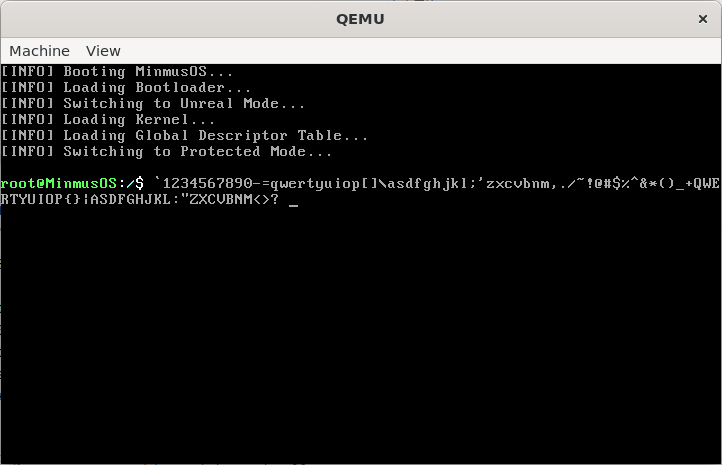
\includegraphics[width=0.8\textwidth]{figures/KeyboardDriverPresentation.png}
    \caption{键盘驱动程序演示}
    \label{fig:KeyboardDriverPresentation}
\end{figure}

\subsubsection{高级技术附件磁盘驱动程序(Advanced Technology Attachment Disk Driver)}

ATA(高级技术附件)磁盘驱动器是一种用于连接存储设备的标准接口,支持硬盘、软盘和光盘驱动器。虽然现代系统中更常见的是使用SATA接口,但ATA接口因其简单性在一些系统中仍被使用。

ATA磁盘驱动程序主要用于控制和管理磁盘读写操作。其核心功能之一是“读取”操作,该操作涉及以下几个步骤:

\begin{enumerate}
    \item \textbf{检查驱动器状态}:在进行读取之前,驱动程序会检查ATA驱动器是否启用并确保其处于非忙碌状态。
    \item \textbf{设置寄存器}:驱动程序设置ATA控制器的寄存器,输入必要的数据,如逻辑块地址(LBA)和要读取的扇区数量。
    \item \textbf{发送读取命令}:驱动程序向控制器发送读取命令,启动数据传输过程。
    \item \textbf{数据传输}:在读取命令发出后,控制器从磁盘读取数据到其内部缓冲区。驱动程序随后通过一个循环,从缓冲区将数据传输到指定的内存位置。由于磁盘的每个扇区大小通常为512字节,而缓冲区可能更小,例如4字节,因此需要多次迭代来完整地传输一个扇区的数据。
    \item \textbf{循环读取}:在每次迭代中,驱动程序都需要检查控制器是否已准备好下一次数据传输,确保不会在数据未完全就绪时进行读取。
\end{enumerate}

这种PIO(程序输入/输出)模式虽然对CPU负担较重,但由于其实现简单,因此在一些基础或旧的系统中仍然被采用。通过使用这种方法,ATA磁盘驱动程序能够有效地管理数据在存储设备与计算机内存之间的传输。

kernel/src/drivers/disk.rs 定义了一个高级技术附件磁盘驱动程序(Advanced Technology Attachment Disk Driver),这个磁盘驱动程序在实现上非常直接,主要通过直接与硬件寄存器交互来控制硬盘操作,而不依赖于操作系统提供的抽象层。

相关常量定义如下:

\begin{enumerate}
    \item \texttt{DATA\_REGISTER}:数据寄存器端口,用于读写数据。当进行数据传输时,数据会通过这个端口传入或传出。
    \item \texttt{SECTOR\_COUNT\_REGISTER}:扇区计数寄存器,用于指定在一个操作中要传输的扇区数量。
    \item \texttt{LBA\_LOW\_REGISTER}:LBA(逻辑块地址)的低位寄存器,用于指定LBA地址的低8位。
    \item \texttt{LBA\_MID\_REGISTER}:LBA(逻辑块地址)的中位寄存器,用于指定LBA地址的中8位。
    \item \texttt{LBA\_HIGH\_REGISTER}:LBA(逻辑块地址)的高位寄存器,用于指定LBA地址的高8位。
    \item \texttt{DRIVE\_REGISTER}:驱动器寄存器,用于选择操作的硬盘和该硬盘的哪个分区。
    \item \texttt{STATUS\_COMMAND\_REGISTER}:状态和命令寄存器。作为命令寄存器时用于发送命令给ATA控制器;作为状态寄存器时用于读取当前的设备状态。
    \item \texttt{READ\_COMMAND}:读取命令的代码,当要从硬盘读取数据时,通过状态命令寄存器发送这个命令。
    \item \texttt{STATUS\_BSY}:状态寄存器中的忙碌位标志,当硬盘忙碌时该位为1。
    \item \texttt{STATUS\_RDY}:状态寄存器中的就绪位标志,当硬盘准备好进行数据传输时该位为1。
\end{enumerate}

Disk 结构体定义了一个简单的 ATA 硬盘驱动程序,并包含多个方法用于硬盘的操作和状态检查。字段 enabled 类型为 bool,标识硬盘是否被启用。

\paragraph{is\_busy方法}

is\_busy 方法的主要功能是检查ATA硬盘的状态,确保在硬盘忙于处理其他命令时不会发起新的操作。这个方法通过查询硬盘的状态寄存器来判断是否有正在执行的任务,从而防止命令冲突和数据损坏。

\cref{lst:IsBusyMethod}使用 Rust 的内联汇编直接从硬盘的状态命令寄存器(STATUS\_COMMAND\_REGISTER)读取状态,特别关注忙碌位(BSY)。方法内部通过检查这个忙碌位是否设置(值为1),来确定硬盘是否处于忙碌状态,并返回相应的布尔值。这种直接与硬件寄存器交互的方式使得该方法既高效又精确。

\begin{listing}[htbp]
    \begin{minted}{rust}
pub fn is_busy(&self) -> bool {
    let status: u8;
    unsafe {
        asm!("in al, dx", out("al") status, in("dx") STATUS_COMMAND_REGISTER);
    }
    (status & STATUS_BSY) != 0
}
    \end{minted}
    \caption{is\_busy方法}\label{lst:IsBusyMethod}
\end{listing}

\paragraph{is\_ready方法}

is\_ready 方法的功能是检查ATA硬盘是否已经准备好接受新的命令。这个方法通过读取硬盘的状态寄存器来判断就绪位(RDY),如果就绪位被设置,表示硬盘处于空闲状态,可以安全地发送新的读写命令。

\cref{lst:IsReadyMethod}利用 Rust 的内联汇编语句从硬盘的状态命令寄存器(STATUS\_COMMAND\_REGISTER)直接读取状态值。方法通过检查就绪位(RDY),这个位在状态寄存器中的特定位置标识硬盘是否准备好进行操作。通过与就绪位掩码(STATUS\_RDY)进行按位与操作来确定硬盘是否就绪,如果结果为真,则返回 true,表示硬盘已经准备好接受新的操作。这种直接操作硬件寄存器的方法确保了检查的及时性和准确性。

\begin{listing}[htbp]
    \begin{minted}{rust}
pub fn is_ready(&self) -> bool {
    let status: u8;
    unsafe {
        asm!("in al, dx", out("al") status, in("dx") STATUS_COMMAND_REGISTER);
    }
    (status & STATUS_RDY) != 0
}
    \end{minted}
    \caption{is\_ready方法}\label{lst:IsReadyMethod}
\end{listing}

\paragraph{check方法}

check 方法的功能是验证ATA硬盘的操作状态,并更新硬盘的启用状态。此方法通过读取状态寄存器,检查硬盘是否正常响应命令,从而确定硬盘是否工作正常。如果状态寄存器的值表明硬盘处于异常状态(如完全不响应或返回错误状态),则硬盘将被标记为禁用。

\cref{lst:CheckMethod}使用 Rust 的内联汇编来直接从硬盘的状态命令寄存器读取当前状态值。通过判断这个状态值是否为 0 或 0xFF(通常表示硬件无响应或通信故障),来决定硬盘是否启用。如果状态值显示硬盘正常(即不是 0 或 0xFF),方法将 enabled 设置为 true 并记录信息日志;反之,设置为 false 并记录错误日志。这种方法可以及时捕捉到硬盘的异常状态,帮助进行故障诊断和维护。

\begin{listing}[htbp]
    \begin{minted}{rust}
pub fn check(&mut self) {
    let status: u8;
    unsafe {
        asm!("in al, dx", out("al") status, in("dx") STATUS_COMMAND_REGISTER);
    }
    if status != 0 && status != 0xFF {
        self.enabled = true;
        lib::println!("[INFO] ATA Disk Driver is Working. Status Register: 0x{:X}", status);
    } else {
        self.enabled = false;
        lib::println!("[ERROR] ATA Disk Driver is not Working! Status Register: 0x{:X}", status);
    }
}
    \end{minted}
    \caption{check方法}\label{lst:CheckMethod}
\end{listing}

\paragraph{reset方法}

reset 方法的主要功能是重置ATA硬盘,将其恢复到初始状态。这个操作对于解决硬盘冻结或响应异常的情况非常有用,通过发送特定的重置命令来清除任何挂起的操作或错误状态,确保硬盘能够重新开始接受命令。

\cref{lst:ResetMethod}通过 Rust 的内联汇编语句直接向硬盘的控制寄存器(位于端口 0x3F6)发送重置命令。具体地,它首先发送一个重置启动的命令(0b00000110),随后发送一个重置结束的命令(0b00000010)。这种直接与硬件寄存器交互的方式确保了命令的即时执行和硬盘状态的即时更新,从而有效地重置硬盘。

\begin{listing}[htbp]
    \begin{minted}{rust}
pub fn reset(&self) {
    unsafe {
        asm!("out dx, al", in("dx") 0x3F6, in("al") 0b00000110u8);
        asm!("out dx, al", in("dx") 0x3F6, in("al") 0b00000010u8);
    }
}
    \end{minted}
    \caption{reset方法}\label{lst:ResetMethod}
\end{listing}

\paragraph{read方法}

read 方法(\cref{lst:ReadMethod})的功能是从ATA硬盘上指定的逻辑块地址(LBA)开始读取一定数量的扇区数据到指定的内存地址。此方法在硬盘已启用且处于空闲状态时执行,通过设置必要的控制寄存器和发送读取命令,逐扇区地从硬盘读取数据并存储到提供的目标内存位置。该方法是硬盘驱动中实现数据读取的核心功能,确保了数据能够安全且有效地从硬盘传输到系统内存中。方法的实现逻辑如下:

\begin{enumerate}
    \item \textbf{检查硬盘是否启用}:方法首先检查 Disk 结构体的 enabled 字段。如果硬盘未启用,则输出错误信息并提前返回,不执行任何读取操作。
    \item \textbf{等待硬盘不忙}:在开始设置命令之前,方法循环调用 is\_busy 方法来确保硬盘不处于忙碌状态。这是必要的步骤,因为如果硬盘正忙于处理其他命令,尝试读取可能会导致命令失败或数据损坏。
    \item \textbf{设置控制寄存器}:使用内联汇编,方法设置了相关的控制寄存器来准备硬盘进行数据读取。
          \begin{enumerate}
              \item \textbf{扇区计数寄存器}:设置要读取的扇区数。
              \item \textbf{LBA 寄存器}:设置逻辑块地址,分为低、中、高位,确保完整的 LBA 地址被正确设置。
              \item \textbf{驱动器寄存器}:设置目标驱动器和LBA的最高位。
              \item \textbf{命令寄存器}:发送读取命令到硬盘。
          \end{enumerate}
    \item \textbf{读取数据}:初始化一个循环,根据指定的扇区数进行迭代。每个扇区通常是 512 字节。对于每个扇区,方法执行另一个循环128次(因为每次从数据寄存器读取4字节,512/4 = 128)。
          \begin{enumerate}
              \item 内部循环先检查硬盘是否忙碌,然后检查是否就绪。
              \item 使用内联汇编从数据寄存器读取4字节数据到本地变量 buffer。
              \item 使用 \texttt{core::ptr::write\_unaligned} 将读取的数据写入目标内存地址,并将目标指针移动4字节以准备下次写入。
          \end{enumerate}
    \item \textbf{重置硬盘}:在所有扇区读取完成后,调用 reset 方法将硬盘重置到初始状态,确保硬盘不会因为留下未完成的命令而出现问题。
\end{enumerate}

\begin{listing}[htbp]
    \begin{minted}{rust}
pub fn read<T>(&self, target: *mut T, lba: u64, sectors: u16) {
    if !self.enabled {
        lib::println!("[ERROR] Failed to Read Disk!");
        return;
    }

    while self.is_busy() {}

    unsafe {
        asm!("out dx, al", in("dx") 0x3F6, in("al") 0b00000010u8);
        asm!("out dx, al", in("dx") SECTOR_COUNT_REGISTER, in("al") sectors as u8);
        asm!("out dx, al", in("dx") LBA_LOW_REGISTER, in("al") lba as u8);
        asm!("out dx, al", in("dx") LBA_MID_REGISTER, in("al") (lba >> 8) as u8);
        asm!("out dx, al", in("dx") LBA_HIGH_REGISTER, in("al") (lba >> 16) as u8);
        asm!("out dx, al", in("dx") DRIVE_REGISTER, in("al") (0xE0 | ((lba >> 24) & 0xF)) as u8);
        asm!("out dx, al", in("dx") STATUS_COMMAND_REGISTER, in("al") READ_COMMAND);
    }

    let mut sectors_left = sectors;
    let mut target_pointer = target;

    while sectors_left > 0 {
        for _i in 0..128 {
            while self.is_busy() {}
            while !self.is_ready() {}
            let buffer: u32;
            unsafe {
                asm!("in eax, dx", out("eax") buffer, in("dx") DATA_REGISTER);
                core::ptr::write_unaligned(target_pointer as *mut u32, buffer);
                target_pointer = target_pointer.byte_add(4);
            }
        }
        sectors_left -= 1;
    }

    self.reset();
}
    \end{minted}
    \caption{read方法}\label{lst:ReadMethod}
\end{listing}

整个方法的实现逻辑既考虑了硬件操作的精确性,也确保了通过适当的检查和等待来避免硬件冲突。这种低级的硬盘操作需要精确控制硬件寄存器,同时确保数据的完整性和正确性。

\cref{fig:ATADiskDriverPresentation}展示了ATA磁盘驱动程序正在工作,且状态寄存器的值为 0x50。状态寄存器的值是一个 8 位的数,在硬盘接口中有特定的含义,每个位代表硬盘的一个不同的状态。对于状态寄存器值 0x50,将其转换为二进制表达为 0101 0000,分析如下:

\begin{enumerate}
    \item \textbf{位 7(BSY)}:0 - 硬盘当前不忙
    \item \textbf{位 6(DRDY)}:1 - 硬盘已准备好接受命令
    \item \textbf{位 5(DF)}:0 - 无设备故障
    \item \textbf{位 4(DSC)}:1 - 设备搜索操作已完成
    \item \textbf{位 3(DRQ)}:0 - 当前没有数据请求
    \item \textbf{位 2(CORR)}:0 - 无已纠正的数据
    \item \textbf{位 1(IDX)}:0 - 在检测到状态的时刻,磁盘的旋转周期没有重新开始
    \item \textbf{位 0(ERR)}:0 - 无错误
\end{enumerate}

\begin{figure}[htbp]
    \centering
    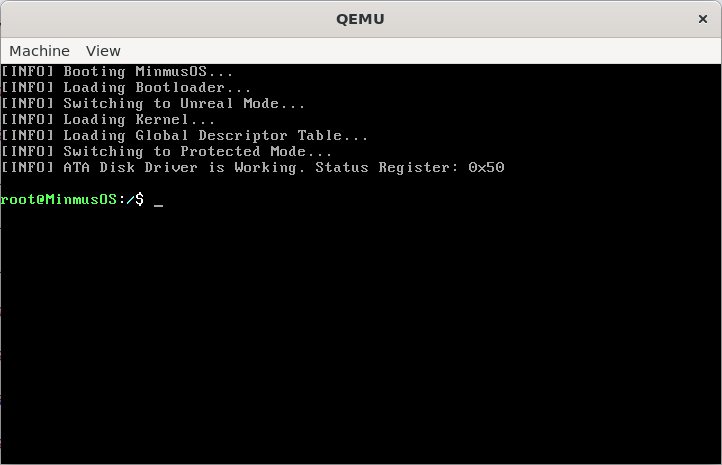
\includegraphics[width=0.8\textwidth]{figures/ATADiskDriverPresentation.png}
    \caption{ATA磁盘驱动程序演示}
    \label{fig:ATADiskDriverPresentation}
\end{figure}

\subsection{多任务处理(Multitasking)}

多任务处理是现代操作系统中一项基本功能,允许单个处理器同时运行多个任务。在单核系统中,虽然物理上不可能真正同时执行多个任务,但通过合理的时间分配,操作系统能够让用户感受到多个任务似乎是在同时运行。这种技术称为“并发”(Concurrency),它与真正的“并行”(Parallelism)不同,后者指的是在多核或多处理器系统中同时执行多个任务。

MinmusOS是一个支持抢占式多任务的操作系统。与协作式多任务系统不同,协作式系统中的任务需要主动放弃CPU使用权,抢占式系统则不需要任务主动放弃处理器。在抢占式系统中,操作系统通过定时器中断来强制从当前任务切换到另一个任务。每当定时器发送中断信号时,中断处理程序会调用调度程序,由调度程序决定下一个要执行的任务。这种方式确保了操作系统能高效地管理CPU资源,响应性好,可以处理大量任务,同时也增强了系统对于紧急处理需求的能力。

\subsubsection{上下文切换(Context Switching)}

在多任务操作系统中,上下文切换是一个至关重要的过程,它使得操作系统能够在多个任务之间高效切换,保证每个任务都能得到适当的处理器时间。上下文切换主要涉及保存当前任务的CPU状态,并在恢复执行另一个任务时加载其之前的状态。这样,即使任务被暂停,稍后恢复时也能如同从未停止过一样继续执行。

上下文的两个主要组成部分是任务栈(Task Stack)和CPU状态(CPU State):

\begin{enumerate}
    \item \textbf{任务栈}:每个任务都有自己的栈,这使得任务可以在需要时由调度器恢复。栈中保存着执行任务所需的所有信息,包括局部变量、函数调用的返回地址等。
    \item \textbf{CPU状态}:包括各种寄存器的值,如程序计数器、堆栈指针、状态寄存器等,这些寄存器的值决定了任务的执行状态。
\end{enumerate}

在 MinmusOS 中,定时器中断(IRQ9)负责在每个定时器滴答时触发调度程序。调度程序的一个关键指令是 mov esp, eax,这条指令将堆栈指针(ESP)设置为从定时器处理程序返回的值。该处理程序返回下一个要执行任务的堆栈指针。由于这个栈的底部包含了旧的CPU状态,所以弹出(popping)CPU寄存器就会恢复到该任务被暂停前的CPU状态。这种机制确保了操作系统能够在多个任务之间平滑且高效地切换,从而实现高度并发的执行,增强了系统的响应性和多任务处理能力。

\cref{lst:TimerFunction}使用了裸函数(\texttt{\#[naked]}),这意味着该函数不会由编译器生成入口和退出代码,完全依赖于程序员手写的汇编代码来控制。这是必须的,因为上下文切换需要精确地控制栈和寄存器的状态。

\begin{listing}[htbp]
    \begin{minted}{rust}
#[naked]
pub extern "C" fn timer() {
    unsafe {
        core::arch::asm!(
        "cli",                // 禁用中断,确保上下文切换不被打断
        "push ebp",           // 保存所有寄存器,以保持当前任务的状态
        "push edi",
        "push esi",
        "push edx",
        "push ecx",
        "push ebx",
        "push eax",
        "push esp",           // 将当前栈指针(esp)压栈,作为参数传递给 C 函数
        "call timer_handler", // 调用 Rust 部分的处理函数
        "mov esp, eax",       // 将 C 函数返回的新栈指针设为当前栈指针
        "pop eax",            // 恢复所有寄存器
        "pop ebx",
        "pop ecx",
        "pop edx",
        "pop esi",
        "pop edi",
        "pop ebp",
        "sti",                // 重新开启中断
        "iretd",              // 从中断返回
        options(noreturn),
        );
    }
}
    \end{minted}
    \caption{timer函数}\label{lst:TimerFunction}
\end{listing}

\cref{lst:TimerHandlerFunction}是上下文切换逻辑的核心。在 timer\_handler 函数中,上下文切换的实现涉及调用任务调度器以选择下一个执行的任务并获取其栈指针,计算该任务在内存中的目标地址,然后更新页表以映射到新的任务地址。这样,当中断处理完成后,CPU可以从新任务的保存状态继续执行,实现任务间的无缝切换。

\begin{listing}[htbp]
    \begin{minted}{rust}
#[no_mangle]
pub extern "C" fn timer_handler(esp: u32) -> u32 {
    unsafe {
        // 调用任务调度器,并传递当前的栈指针,返回新任务的栈指针
        let new_esp: u32 = TASK_MANAGER.schedule(esp as *mut CPUState) as u32;
        // 获取当前任务的槽位
        let slot = TASK_MANAGER.get_current_slot();
        // 计算当前任务的内存目标地址
        let target = APP_TARGET + (slot as u32 * APP_SIZE);
        // 更新页表,将任务的代码映射到正确内存位置,确保 CPU 在执行新任务时访问到正确的代码和数据
        TABLES[8].set(target);
        // 使页表更改生效
        PAGING.set_table(8, &TABLES[8]);
        // 发送中断结束信号到 PIC,告知中断处理完成
        PICS.end_interrupt(TIMER_INT);
        // 返回新的栈指针
        new_esp
    }
}
    \end{minted}
    \caption{timer\_handler函数}\label{lst:TimerHandlerFunction}
\end{listing}

这种结合汇编和高级语言的方式允许操作系统精确控制硬件,实现高效的多任务处理和上下文切换。通过这样的实现,即使在单核处理器上,操作系统也能够提供平滑的多任务环境。

\subsubsection{CPU 调度器(CPU Scheduler)}\label{sec:CPUScheduler}

MinmusOS 使用了轮转调度(round robin)算法来管理任务的调度,该算法通过定时器中断处理程序触发。每当发生一个定时器滴答,调度算法就会从任务列表中选择下一个任务,并返回一个指向该任务CPU状态的指针。

这个返回的指针非常关键,因为它指向了被选择任务的CPU状态。在上下文切换时,上下文切换器会将栈指针设置为这个指针,并从中弹出(pop)寄存器的值,以此恢复任务的状态。这样,当任务再次运行时,就可以从上次停止的地方继续执行,实现任务间的平滑切换。

轮转调度(Round Robin, RR)算法是一种非常常见的任务调度方法,尤其适用于时间分片的操作系统中。在RR算法中,每个任务被赋予一个固定时间的时间片或量子(quantum),所有任务按照一定的顺序排列,形成一个循环队列。

轮转调度算法的主要特点和步骤包括:

\begin{enumerate}
    \item \textbf{时间片}:系统为每个任务分配一个固定长度的时间片,这是任务可以连续运行的最大时间。时间片的长度通常由操作系统确定,需要平衡响应时间和系统效率。
    \item \textbf{任务切换}:当一个任务的时间片用完时,如果它还没有完成,则会被操作系统挂起。调度器将CPU控制权转移给队列中的下一个任务。
    \item \textbf{循环队列}:所有等待运行的任务形成一个循环队列。调度器按照队列的顺序为每个任务分配CPU时间,一旦到达队列末尾,调度器就从队列头开始新一轮的任务调度。
    \item \textbf{公平性}:RR算法的一个显著优点是它的公平性。每个任务都有相同长度的时间运行,这意味着没有单个任务能长时间独占CPU,从而保证了所有任务都能获得足够的处理时间。
    \item \textbf{响应时间}:由于任务经常被切换,RR算法能提供较好的响应时间,适合需要频繁交互的应用。但是,频繁的任务切换也可能导致较高的开销,因为每次切换都需要进行上下文保存和恢复。
\end{enumerate}

轮转调度算法适用于多任务环境,尤其是处理许多短任务的系统。通过合理设置时间片长度,可以使系统达到良好的性能平衡。

\begin{listing}[htbp]
    \begin{minted}{rust}
pub fn schedule(&mut self, cpu_state: *mut CPUState) -> *mut CPUState {
    if self.task_count <= 0 {
        return cpu_state;
    }
    if self.current_task >= 0 {
        self.tasks[self.current_task as usize].cpu_state_ptr = cpu_state as u32;
    }
    self.current_task = self.get_next_task();
    self.tasks[self.current_task as usize].cpu_state_ptr as *mut CPUState
}

pub fn get_next_task(&self) -> i8 {
    let mut i = self.current_task + 1;
    while i < MAX_TASKS {
        if self.tasks[i as usize].running {
            return i;
        }
        i = (i + 1) % MAX_TASKS;
    }
    -1
}
    \end{minted}
    \caption{轮转调度(Round Robin, RR)算法}\label{lst:RoundRobinAlgorithm}
\end{listing}

\cref{lst:RoundRobinAlgorithm}通过两个主要函数 schedule 和 get\_next\_task 来实现轮转调度算法。schedule 函数首先检查是否有任务在运行,如果有,它会保存当前任务的CPU状态。然后,它调用 get\_next\_task 函数,从任务列表中按顺序选择下一个可运行的任务,并返回该任务的CPU状态指针,供系统加载和执行。

get\_next\_task 函数实现了任务的轮转选择逻辑。它从当前任务的下一个任务开始查找,直到找到一个正在运行的任务。如果到达任务列表末尾,它会循环回到列表的开头,继续查找。如果找不到任何运行的任务,则返回 -1。

这种实现方式确保了所有任务都能依次得到执行机会,公平地分配CPU时间,符合轮转调度算法的特点。

\subsubsection{任务管理器(Task Manager)}

任务管理器(Task Manager)是操作系统中负责管理任务的组件,主要职责包括插入、移除和调度任务。任务管理器由多个函数组成,用于操作任务列表,并包含一个数据结构,存储任务数组、任务数量以及当前正在运行任务的ID。

\paragraph{\texttt{CPUState}数据结构}

CPUState 是一个表示 CPU 状态的结构体(\cref{lst:CPUStateDataStructure}),使用 \texttt{\#[repr(C, packed)]} 属性确保其在内存中的布局与 C 语言的结构体一致且紧密排列。这个结构体保存了寄存器的状态,其中包括手动压入栈的寄存器(如 eax, ebx, ecx, edx, esi, edi, ebp)和 CPU 自动压入的寄存器(如 eip, cs, eflags, esp, ss)。这些寄存器的值通常在上下文切换或异常处理中被保存和恢复,以确保线程或异常处理返回时能够继续正确的执行。

\begin{listing}[htbp]
    \begin{minted}{rust}
#[repr(C, packed)]
pub struct CPUState {
    eax: u32,
    ebx: u32,
    ecx: u32,
    edx: u32,
    esi: u32,
    edi: u32,
    ebp: u32,
    eip: u32,
    cs: u32,
    eflags: u32,
    esp: u32,
    ss: u32,
}
    \end{minted}
    \caption{\texttt{CPUState}数据结构}\label{lst:CPUStateDataStructure}
\end{listing}

\paragraph{\texttt{Task}数据结构}

Task 结构体(\cref{lst:TaskDataStructure})表示操作系统中的一个任务。它包含了任务运行所需的关键信息,包括一个固定大小的栈 stack,一个指向 CPU 状态保存位置的指针 cpu\_state\_ptr,以及一个布尔值 running,用于表示任务是否正在运行。stack 用于存储任务的局部变量和函数调用信息,而 cpu\_state\_ptr 指向 CPUState 结构体,以保存任务的寄存器状态,方便在任务切换时进行恢复。

\begin{listing}[htbp]
    \begin{minted}{rust}
#[derive(Copy, Clone, Debug)]
pub struct Task {
    pub stack: [u8; STACK_SIZE],
    pub cpu_state_ptr: u32,
    pub running: bool,
}

impl Task {
    pub fn init(&mut self, entry_point: u32) {
        self.running = true;
        let mut state = &self.stack as *const u8;
        unsafe {
            state = state.byte_add(STACK_SIZE);
            state = state.byte_sub(size_of::<CPUState>());
        }
        self.cpu_state_ptr = state as u32;
        let cpu_state = self.cpu_state_ptr as *mut CPUState;
        unsafe {
            (*cpu_state).eax = 0;
            (*cpu_state).ebx = 0;
            (*cpu_state).ecx = 0;
            (*cpu_state).edx = 0;
            (*cpu_state).esi = 0;
            (*cpu_state).edi = 0;
            (*cpu_state).ebp = 0;
            (*cpu_state).eip = entry_point;
            (*cpu_state).cs = 0x8;
            (*cpu_state).eflags = 0x202;
        }
    }
}
    \end{minted}
    \caption{\texttt{Task}数据结构}\label{lst:TaskDataStructure}
\end{listing}

Task 结构体实现了一个 init 方法,用于初始化任务。初始化过程中,将 running 标记为 true,表示任务开始运行。然后计算 CPUState 的位置,cpu\_state\_ptr 指向栈顶减去 CPUState 大小的位置,确保 CPUState 有足够的空间存储在栈中。接着,初始化 CPUState 结构体中的各个寄存器值:

\begin{enumerate}
    \item \textbf{通用寄存器(eax, ebx, ecx, edx, esi, edi, ebp)}:设置为 0,以保证任务开始时寄存器处于已知状态。
    \item \textbf{程序计数器(eip)}:设置为传入的 entry\_point,表示任务从这个地址开始执行。entry\_point 是任务的入口地址,通常指向任务的第一条指令。
    \item \textbf{代码段寄存器(cs)}:设置为 0x8,这是一个常见的代码段选择子,通常在操作系统中表示内核代码段。
    \item \textbf{标志寄存器(eflags)}:设置为 0x202。0x202 表示启用了中断(IF 位为 1),并且设置了固定的保留位。这样可以确保任务在开始执行时,CPU的标志状态正确。
\end{enumerate}

NULL\_TASK 是一个静态变量(\cref{lst:NullTaskStaticVariable}),用作任务的默认空白模板,表示未初始化或未运行的任务。它的 stack 被初始化为全零,cpu\_state\_ptr 为 0,running 标志设置为 false。NULL\_TASK 在创建新任务时作为基础,并通过调用 init 方法进行具体的初始化,避免每次创建任务时都手动构建任务结构体。

\begin{listing}[htbp]
    \begin{minted}{rust}
static NULL_TASK: Task = Task {
    stack: [0; STACK_SIZE],
    cpu_state_ptr: 0u32,
    running: false,
};
    \end{minted}
    \caption{NULL\_TASK静态变量}\label{lst:NullTaskStaticVariable}
\end{listing}

\paragraph{\texttt{TaskManager}数据结构}

TaskManager 是一个管理操作系统中所有任务的结构体(\cref{lst:TaskManagerDataStructure})。它包含以下几个重要字段:

\begin{enumerate}
    \item \texttt{tasks}:一个固定大小的数组,用于存储系统中的所有任务。数组的大小由常量 MAX\_TASKS 决定,每个元素都是一个 Task 结构体实例。
    \item \texttt{task\_count}:记录当前运行的任务数量。
    \item \texttt{current\_task}:表示当前正在执行的任务的索引。使用 -1 表示没有当前任务或系统处于空闲状态。
\end{enumerate}

\begin{listing}[htbp]
    \begin{minted}{rust}
pub struct TaskManager {
    tasks: [Task; MAX_TASKS as usize],
    task_count: i8,
    current_task: i8,
}

impl TaskManager {
    pub fn init(&mut self) {
        self.add_task(idle as u32);
    }

    pub fn add_task(&mut self, entry_point: u32) {
        self.tasks[self.get_free_slot() as usize].init(entry_point);
        self.task_count += 1;
    }

    pub fn remove_task(&mut self, id: usize) {
        if id != 0 {
            self.tasks[id] = NULL_TASK;
            self.task_count -= 1;
        }
    }

    pub fn remove_current_task(&mut self) {
        self.remove_task(self.current_task as usize);
    }

    pub fn schedule(&mut self, cpu_state: *mut CPUState) -> *mut CPUState { ... }

    pub fn get_next_task(&self) -> i8 { ... }

    pub fn get_free_slot(&self) -> i8 {
        let mut slot: i8 = -1;
        for i in 0..MAX_TASKS {
            if self.tasks[i as usize].running == false {
                slot = i;
                return slot;
            }
        }
        slot
    }

    pub fn get_current_slot(&self) -> i8 {
        self.current_task
    }

    pub fn list_tasks(&self) {
        lib::println!("Running tasks:");
        for i in 0..MAX_TASKS {
            if self.tasks[i as usize].running {
                lib::println!("PID: {}", i);
            }
        }
    }
}
    \end{minted}
    \caption{\texttt{TaskManager}数据结构}\label{lst:TaskManagerDataStructure}
\end{listing}

TaskManager 的方法实现如下:

\begin{enumerate}
    \item \texttt{init}:添加一个空闲任务(idle),以确保即使没有其他任务运行,系统也有一个默认任务执行。idle 函数是一个空闲任务,在一个无限循环中执行 hlt 指令,以使 CPU 进入低功耗状态,等待外部中断恢复。
    \item \texttt{add\_task}:向任务管理器中添加一个新任务。它会先找到一个空闲的任务槽(未使用的 Task 实例),然后初始化该任务,并将 task\_count 计数器加 1。
    \item \texttt{remove\_task}:删除指定 ID 的任务。该方法会重置任务槽为 NULL\_TASK,并减少任务数量。
    \item \texttt{remove\_current\_task}:删除当前正在运行的任务。它调用 remove\_task 方法,并传入当前任务的 ID。
    \item \texttt{schedule}和\texttt{get\_next\_task}:通过轮转调度算法进行任务调度。保存当前任务的 CPU 状态,然后选择下一个任务并返回其 CPU 状态指针,具体实现见\cref{sec:CPUScheduler},在此不再赘述。
    \item \texttt{get\_free\_slot}:找到第一个空闲任务槽的索引。如果没有找到空闲槽,返回 -1。
    \item \texttt{get\_current\_slot}:返回当前正在运行的任务的索引。
    \item \texttt{list\_tasks}:列出所有正在运行的任务的 PID。
\end{enumerate}

TASK\_MANAGER 静态变量(\cref{lst:TaskManagerStaticVariable})是整个操作系统中唯一的 TaskManager 实例,用于全局管理所有的任务。它的作用包括:

\begin{listing}[htbp]
    \begin{minted}{rust}
pub static mut TASK_MANAGER: TaskManager = TaskManager {
    tasks: [NULL_TASK; MAX_TASKS as usize],
    task_count: 0,
    current_task: -1,
};
    \end{minted}
    \caption{TASK\_MANAGER静态变量}\label{lst:TaskManagerStaticVariable}
\end{listing}

\begin{enumerate}
    \item \textbf{任务管理的核心控制}:跟踪和调度系统中的所有任务。它持有任务列表(tasks),管理当前任务的状态(current\_task),并记录系统中总共存在的任务数量(task\_count)。
    \item \textbf{提供全局访问}:系统中各个部分可以方便地访问这个任务管理器,这对于任务调度、任务创建、删除、切换等操作非常重要。
    \item \textbf{任务初始化和调度}:在系统启动时初始化默认任务(例如 idle 任务),并在系统运行过程中负责调度各个任务。这使得操作系统能够在多任务环境下正确地进行任务切换,确保系统的稳定运行。
    \item \textbf{持久存在的状态管理}:作为静态变量,TASK\_MANAGER 的生命周期贯穿整个系统的运行期,它的状态在整个操作系统运行过程中是持久的。这意味着任务的状态不会在函数调用结束时丢失,可以在任意时间点被访问和修改。
\end{enumerate}

\subsection{系统调用(System Calls)}

在MinmusOS中,kernel/src/syscalls/handler.rs文件(\cref{lst:HandlerRust})负责处理系统调用。系统调用是用户空间中的程序请求内核服务的一种方式。通过这个接口,内核可以建立一个安全模型,对某些进程可以执行的操作类型和范围进行限制,它是内核功能对用户空间的一种暴露。

在MinmusOS中,系统调用通过\texttt{syscall()}函数使用软件中断(中断向量0x80)来触发。这种机制类似于Linux在x86架构上使用的方法。

目前,MinmusOS只支持两个系统调用:

\begin{enumerate}
    \item \textbf{系统调用0}:打印由EBX寄存器指向的地址开始的字符串,长度由ECX寄存器指定。
    \item \textbf{系统调用1}:从任务列表中移除当前运行的任务。
\end{enumerate}

以下是处理系统调用的关键步骤:

\begin{enumerate}
    \item \textbf{中断触发和保存寄存器}:使用\texttt{asm!}宏定义的\texttt{syscall()}函数负责保存寄存器状态并调用\texttt{syscall\_handler()}函数。这里eax,ebx和ecx寄存器被推入堆栈,并在调用完\texttt{syscall\_handler}之后恢复,最后执行\texttt{iretd}从中断返回。在\texttt{syscall()}函数中,eax,ebx和ecx寄存器的值被依次推入栈中,每个寄存器都是32位,即4字节。所以,总共推入了12字节。函数执行结束后,需要将这些值从栈上移除,以恢复调用前的栈状态。这就是\texttt{add esp, 12}的作用:它通过增加esp的值来“弹出”这些值,即将栈指针向上移动12字节,回到调用\texttt{syscall\_handler}函数之前的位置。
    \item \textbf{处理系统调用}:\texttt{syscall\_handler()}函数接收来自eax,ebx和ecx寄存器的值作为参数,这些寄存器在\texttt{syscall()}中被传递。eax用于指定系统调用的类型,ebx和ecx用于传递额外的参数或数据。
    \item \textbf{系统调用的分发}:通过检查eax寄存器的值来确定要执行的具体系统调用。
          \begin{enumerate}
              \item \textbf{系统调用0}:打印字符串。通过ebx寄存器传递的地址读取字符串,ecx指定字符串的长度。使用Rust的\texttt{slice::from\_raw\_parts()}和\texttt{str::from\_utf8()}将字节转换为字符串。
              \item \textbf{系统调用1}:移除当前活动任务,通过调用任务管理器的\texttt{remove\_current\_task()}方法来实现。
          \end{enumerate}
    \item \textbf{结束中断处理}:调用\texttt{PICS.end\_interrupt()}方法,标志着对此次中断的处理已经完成,可以继续执行其他操作。
\end{enumerate}

\begin{listing}[htbp]
    \begin{minted}{rust}
#[naked]
pub extern "C" fn syscall() {
    unsafe {
        asm!(
        "push eax",
        "push ebx",
        "push ecx",
        "call syscall_handler",
        "add esp, 12",
        "iretd",
        options(noreturn),
        );
    }
}

#[no_mangle]
pub extern "C" fn syscall_handler(ecx: u32, ebx: u32, eax: u32) {
    unsafe {
        match eax {
            0 => {
                let s = {
                    let slice = slice::from_raw_parts(ebx as *const u8, ecx as usize);
                    str::from_utf8(slice)
                };
                print::PRINTER.prints(s.unwrap());
            }
            1 => {
                TASK_MANAGER.remove_current_task();
            }
            _ => {}
        }
        PICS.end_interrupt(SYSCALL_INT);
    }
}
    \end{minted}
    \caption{kernel/src/syscalls/handler.rs}\label{lst:HandlerRust}
\end{listing}

通过这种方式,MinmusOS能够提供一种有效且安全的机制,允许用户程序执行核心级的操作,如IO操作和任务管理。

\subsection{VGA模式(Video Graphics Array Mode)}

\subsection{命令行解释器(Shell)}

\subsection{内存管理(Memory Management)}

\subsection{文件系统(File System)}